
\section{\label{sec:Fixedpt}Iterasi Titik Tetap\index{metode iterasi titik tetap}
\index{metode!iterasi titik tetap|see{metode iterasi titik tetap}}}

Ambil kalkulator Anda. Kalkulator apa pun yang memiliki tombol kosinus
sudah memadai. Jika Anda menggunakan kalkulator ilmiah sederhana,
tekan tombol hapus semua, yang biasanya bertanda \texttt{AC} atau
cukup \texttt{C}. Layar kini seharusnya menampilkan 0. Tekan tombol
kosinus, yang seharusnya bertanda \texttt{cos}. Layar seharusnya menampilkan
1. Tekan lagi tombol kosinus. Layar seharusnya menampilkan $0.540302\ldots$.
Ulangi. Ulangi lagi. Bahkan, teruslah menekan tombol kosinus sampai
Anda melihat suatu pola. 

Jika Anda memiliki kalkulator yang lebih canggih dengan tombol jawaban
sebelumnya, biasanya bertanda \texttt{Ans}, tekan 0 lalu \texttt{Enter}
atau \texttt{=}. Kemudian tekan tombol kosinus lalu tombol jawaban
sebelumnya. Setelah itu, tekan \texttt{Enter} atau \texttt{=} untuk
melakukan perhitungan. Pada kali pertama, layar seharusnya menampilkan
1 (sama seperti pada kalkulator ilmiah). Namun, untuk mengulanginya,
cukup tekan \texttt{Enter} atau \texttt{=} lagi. Tindakan ini akan
mengulangi perhitungan terakhir, yaitu kosinus dari jawaban sebelumnya.
Layar seharusnya menampilkan $0.540302\ldots$. Sekarang ulangi sampai
Anda melihat suatu pola.

Setelah sekitar 30 pengulangan, atau yang akan kita sebut iterasi\index{iterasi},
kalkulator Anda seharusnya menampilkan bilangan seperti $0.739083847\ldots$.
Berapa kali pun Anda mengulangi, atau mengiterasi, perhitungan itu,
nilainya tidak akan banyak berubah. Bahkan, setelah mencapai $0.7390851332\ldots$,
nilainya tidak akan berubah sama sekali (kecuali kalkulator Anda menampilkan
lebih banyak tempat desimal---setelah sekitar 90 iterasi, kalkulator
yang menampilkan 15 tempat desimal akan menunjukkan $0.739085133215161$
dan nilainya tidak akan berubah lagi). Artinya, $\cos(0.7390851332\ldots)=0.7390851332\ldots$.
Kita menyebut $0.7390851332\ldots$ sebagai \index{titik tetap} titik
tetap dari fungsi kosinus. Nilai itu tetap (tidak berubah) ketika
fungsi kosinus diterapkan. Dengan kata lain, pada $0.7390851332\ldots$,
masukan dan keluaran fungsi kosinus sama. Lihat simulasi iterasi ini
secara daring di \href{http://lqbrin.github.io/tea-time-numerical/ancillaries.html}{situs pendamping}.

Barangkali sekarang muncul serangkaian pertanyaan. Mengapa ini berhasil?
Bagaimana jika kita mulai dengan bilangan selain 0? Apakah ini berhasil
untuk sembarang fungsi? Dapatkah kita meramalkan kapan cara ini akan
berhasil atau tidak? Dapatkah kita mencari akar dengan cara ini? Apakah
kekonvergenannya cepat? Dalam bagian ini dan bagian berikutnya, kita
akan memberikan setidaknya jawaban parsial untuk semua pertanyaan
tersebut. Kita mulai dengan ``Mengapa ini berhasil?''.

Perhatikan penyelesaian sistem 
\[
\begin{cases}
y=\cos(x)\\
y=x
\end{cases}.
\]
Salah satu cara menyelesaikannya adalah dengan metode substitusi.
Jika kita menyubstitusikan $y=x$ ke dalam $y=\cos x$ kita memperoleh
$x=\cos x$ atau $\cos x=x$. Solusi sistem tersebut tepat berimpit
dengan titik-titik tetap fungsi kosinus, karena setiap solusi $\cos x=x$
merupakan nilai $x$ yang tidak berubah oleh fungsi kosinus. Karena
sistem dua persamaan dengan dua peubah dapat diselesaikan, setidaknya
secara hampiran, dengan menggambar grafik, hal ini menyarankan agar
kita melihat grafik sistem tersebut untuk memahami lebih jauh apa
yang terjadi selama iterasi.

\begin{figure}[h]
\caption{\label{fig:cosine-fixed-point}Menentukan titik tetap $\cos(x)$.}

\bigskip{}

\centering{}%
\begin{tabular}{cccc}
(a) &  & (b) & \tabularnewline
 & 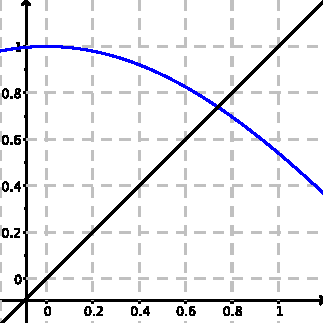
\includegraphics{figures/roots-fixedpt5} &  & 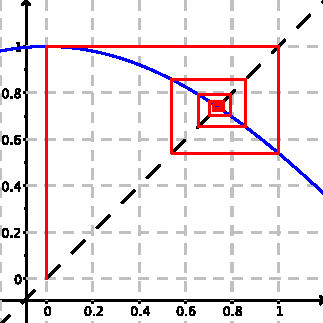
\includegraphics{figures/roots-fixedpt1}\tabularnewline
\end{tabular}
\end{figure}
Gambar \ref{fig:cosine-fixed-point}(a) memperlihatkan grafik $y=\cos(x)$
dan $y=x$ pada interval $[0,1]$. Kita dapat melihat titik potong
di sekitar $(0.75,0.75)$ sehingga kita patut menduga bahwa titik
tetapnya berada di sekitar $0.75$ (yang tentu saja kita ketahui benar
dari percobaan kalkulator). Gambar \ref{fig:cosine-fixed-point}(b)
menggambarkan proses menghitung $\cos(0),\cos(1),\cos(0.540302\ldots),\ldots$.
Menelusuri ruas garis vertikal dari $(0,0)$ ke $(0,1)$ menunjukkan
perhitungan $\cos(0)$. Menelusuri kelanjutan horizontal dari $(0,1)$
ke $(1,1)$ lalu ruas garis vertikal dari $(1,1)$ ke $(1,0.540302\ldots)$
menunjukkan perhitungan $\cos(1)$. Menelusuri garis horizontal dari
$(1,0.540302\ldots)$ ke $(0.540302\ldots,0.540302\ldots)$ lalu garis
vertikal dari $(0.540302\ldots,0.540302\ldots)$ ke $(0.540302\ldots,0.857553\ldots)$
menunjukkan perhitungan $\cos(0.540302\ldots)$, dan seterusnya. Setiap
pasangan ruas garis---yang satu bergerak horizontal dari grafik $y=\cos(x)$
menuju grafik $y=x$ dan yang lain bergerak vertikal dari garis $y=x$
menuju grafik $y=\cos(x)$---menunjukkan satu iterasi lagi. Gambar
\ref{fig:cosine-fixed-point}(b) kadang disebut diagram jaring\index{diagram jaring}
\cite{barnsley}, dan lazim digunakan untuk menggambarkan konsep iterasi.
Lintasan diagram jaring yang menuju $(0.739085\ldots,0.739085\ldots)$
merupakan akibat tak terhindarkan dari geometri grafik $\cos(x)$.

Bagaimana jika kita mulai dengan bilangan selain 0? Dengan menggunakan
Gambar \ref{fig:cosine-fixed-point}, Anda seharusnya dapat meyakinkan
diri bahwa kekonvergenan menuju titik $(0.7390851332\ldots,0.7390851332\ldots)$
terjamin untuk setiap nilai awal antara 0 dan 1. Cobalah. Mulailah
dari sembarang titik pada garis $y=x$. Bergeraklah secara vertikal
ke grafik $y=\cos(x)$. Lalu bergeraklah secara horizontal ke garis
$y=x$. Ulangi. Anda akan mendapati bahwa lintasan diagram jaring
selalu menuju perpotongan kedua grafik. Sekarang pertimbangkan untuk
memulai dengan sembarang bilangan real, $r$. Kosinus setiap bilangan
real berada dalam interval $[-1,1]$ sehingga $\cos(r)\in[-1,1]$.
Kosinus setiap bilangan dalam interval $[-1,1]$ berada dalam interval
$[0,1]$ sehingga $\cos(\cos(r))\in[0,1]$. Artinya, iterasi kedua
berada dalam interval dari 0 sampai 1. Jadi, hanya setelah dua iterasi,
setiap nilai awal akan menjadi nilai antara 0 dan 1. Diagram jaring
kita menunjukkan bahwa iterasi selanjutnya akan menuju titik tetap.
Jadi, apa pun nilai awalnya, iterasi menuju titik tetap. Argumen sebelumnya
menjadi cikal bakal bukti fakta ini.

Namun, tidak semua fungsi berperilaku sebaik itu. Sebagai contoh,
$1^{2}=1$. Dengan kata lain, $1$ adalah titik tetap fungsi $y=x^{2}$.
Akan tetapi, iterasi yang dimulai dari sembarang bilangan selain $1$
atau $-1$ tidak menuju titik tetap ini. Jika kita mulai dengan sembarang
bilangan yang lebih besar dari 1 lalu menguadratkannya, nilainya menjadi
lebih besar. Jika hasilnya dikuadratkan, nilainya menjadi lebih besar
lagi. Menguadratkannya sekali lagi hanya memperbesar nilai tersebut
tanpa batas. Oleh karena itu, iterasi yang dimulai dari sembarang
nilai yang lebih besar dari 1 (atau lebih kecil dari $-1$) tidak
konvergen ke titik tetap $1$. Demikian pula iterasi yang dimulai
dari sembarang bilangan yang nilai mutlaknya kurang dari 1. Gambar
\ref{fig:quadratic-fixed-point} 
\begin{figure}[h]
\caption{\label{fig:quadratic-fixed-point}Memvisualisasikan iterasi $f(x)=x^{2}$.}

\bigskip{}

\centering{}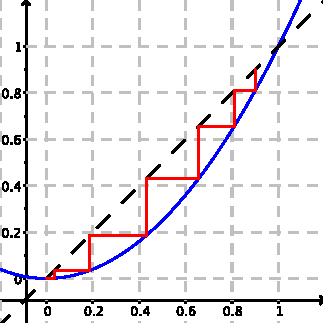
\includegraphics[scale=1.2]{figures/roots-fixedpt2}
\end{figure}
 menggambarkan iterasi $y=x^{2}$ dengan nilai awal $0.9$. Ikuti
diagram jaring dari titik $(0.9,0.9)$ secara vertikal ke grafik $y=x^{2}$
lalu secara horizontal kembali ke garis $y=x$, dan seterusnya, untuk
memeriksanya sendiri. Ini menggambarkan dengan baik fakta bahwa kuadrat
setiap bilangan yang terletak ketat antara 0 dan 1 lebih kecil daripada
bilangan itu sendiri. Untuk nilai awal antara $-1$ dan $1$, dengan
mengecualikan $\pm1$, iterasi menghasilkan barisan yang konvergen
ke 0, bukan 1. Singkatnya, selain $-1$ dan 1, tidak ada nilai awal
yang menghasilkan barisan yang konvergen ke 1 di bawah iterasi fungsi
$y=x^{2}$.

Terdapat perbedaan mendasar antara titik tetap $0.7390851332\ldots$
dari $f(x)=\cos(x)$ dan titik tetap $1$ dari $g(x)=x^{2}$. Iterasi
titik tetap konvergen ke $0.7390851332\ldots$ di bawah $f(x)=\cos(x)$
untuk sembarang nilai awal. Iterasi titik tetap gagal konvergen ke
$1$ di bawah $g(x)=x^{2}$ untuk semua nilai awal kecuali $\pm1$.\footnote{Untuk jenis perilaku ketiga, iterasi titik tetap konvergen ke $0$
di bawah $g(x)$ untuk nilai awal di dekat 0, tetapi tidak untuk nilai
awal lainnya!} Memeriksa grafik $f(x)$ dan $g(x)$ yang masing-masing ditumpangtindihkan
dengan garis $y=x$ di lingkungan titik tetapnya dapat memberi petunjuk
{[}Gambar \ref{fig:fixed-pt-zoom}{]} tentang perbedaannya. 
\begin{figure}[h]
\caption{\label{fig:fixed-pt-zoom}Kiri: \textcolor{blue}{$f(x)=\cos(x)$}
dan $y=x$. Kanan: \textcolor{blue}{$g(x)=x^{2}$} dan $y=x$. }

\bigskip{}

\centering{}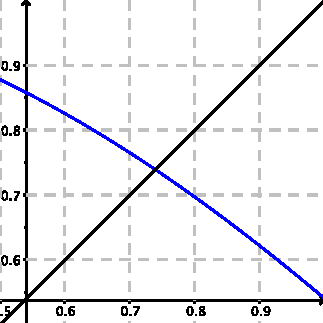
\includegraphics{figures/roots-fixedpt3} 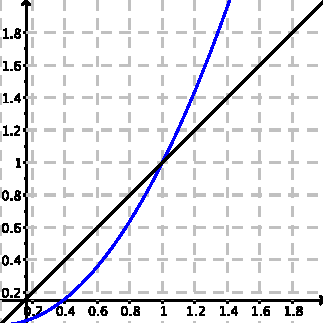
\includegraphics{figures/roots-fixedpt4}
\end{figure}
Memang, $f(x)$ memiliki gradien negatif di titik tetapnya, sedangkan
$g(x)$ memiliki gradien positif di titik tetapnya. Anda dapat melihatnya
dari grafik atau ``melakukan kalkulusnya''. Namun, perbedaan yang
penting lebih halus. Bukan tanda gradien di titik tetap yang menentukan.
Nilai mutlak gradien di titik tetaplah yang menentukan. Untuk fungsi
mulus, lingkungan titik-titik dengan nilai mutlak gradien lebih besar
dari 1 cenderung ekspansif. Artinya, titik-titik saling menjauh ketika
fungsi diterapkan. Sebaliknya, lingkungan titik-titik dengan nilai
mutlak gradien kurang dari 1 cenderung kontraktif. Artinya, titik-titik
saling mendekat ketika fungsi diterapkan. 
\begin{prop}
\label{prop:contractive}Jika $h(x)$ dapat didiferensialkan pada
$(a,b)$ dengan $|h'(x)|<1$ untuk semua $x\in(a,b)$, maka untuk
setiap $x_{1},x_{2}\in(a,b)$, $|h(x_{2})-h(x_{1})|<|x_{2}-x_{1}|$.
\end{prop}

\begin{proof}
Ambil $x_{1},x_{2}\in(a,b)$ dan, tanpa mengurangi keumuman, ambil
$x_{2}>x_{1}$ agar kita dapat dengan tepat merujuk pada interval
dari $x_{1}$hingga $x_{2}$. Karena $h(x)$ kontinu pada $[x_{1},x_{2}]$
dan dapat didiferensialkan pada $(x_{1},x_{2})$, Teorema Nilai Rata-Rata
memberi kita $c\in(x_{1},x_{2})\subseteq(a,b)$ sedemikian sehingga
$h'(c)=\left|\frac{h(x_{2})-h(x_{1})}{x_{2}-x_{1}}\right|$. Namun,
$h'(c)<1$ menurut asumsi, sehingga $h'(c)=\left|\frac{h(x_{2})-h(x_{1})}{x_{2}-x_{1}}\right|<1$,
yang langsung memberikan $|h(x_{2})-h(x_{1})|<|x_{2}-x_{1}|$.
\end{proof}
Selain itu, fungsi yang nilai mutlak turunannya kurang dari 1 hanya
dapat memotong garis $y=x$ satu kali. Setelah memotongnya, fungsi
tersebut tidak pernah dapat ``menyusul'' karena hal itu membutuhkan
gradien yang lebih besar dari 1, yaitu gradien garis $y=x$. 
\begin{prop}
\label{prop:uniquenessOfFixedPoint}Misalkan $h(x)$ kontinu pada
$[a,b]$, dapat didiferensialkan pada $(a,b)$ dengan $|h'(x)|<1$
untuk semua $x\in(a,b)$, dan $h([a,b])\subseteq[a,b]$. Maka $h$
mempunyai tepat satu titik tetap dalam $[a,b]$.
\end{prop}

\begin{proof}
Jika $h(a)=a$ atau $h(b)=b$, keberadaan telah terbukti. Karena itu,
misalkan $h(a)\neq a$ dan $h(b)\neq b$. Karena $h([a,b])\subseteq[a,b]$
harus berlaku $h(a)>a$ dan $h(b)<b$. Langsung diperoleh $h(a)-a>0$
dan $h(b)-b<0$. Karena fungsi bantu $f(x)=h(x)-x$ kontinu pada $[a,b]$,
Teorema Nilai Antara menjamin adanya $c\in(a,b)$ sedemikian sehingga
$f(c)=0$. Dengan substitusi, $h(c)-c=0$, yang menyiratkan $h(c)=c$,
sehingga $c$ adalah titik tetap $h$. Keberadaan titik tetap telah
terbukti. Sekarang misalkan $c_{1}\in[a,b]$ dan $c_{2}\in[a,b]$
adalah titik-titik tetap yang berbeda dari $h$. Maka 
\[
\frac{h(c_{1})-h(c_{2})}{c_{1}-c_{2}}=\frac{c_{1}-c_{2}}{c_{1}-c_{2}}=1.
\]
 Berdasarkan Teorema Nilai Rata-Rata, terdapat $c_{3}$ di antara
$c_{1}$ dan $c_{2}$ sedemikian sehingga $h'(c_{3})=1$, yang bertentangan
dengan fakta bahwa $|h'(x)|<1$ untuk semua $x\in(a,b)$. Oleh karena
itu, tidak mungkin $c_{1}$ dan $c_{2}$ berbeda.
\end{proof}
Jadi, kita dapat secara wajar menduga bahwa jika nilai mutlak turunan
di suatu titik tetap kurang dari 1, iterasi merupakan metode yang
layak untuk menghampiri (menentukan) titik tetap tersebut, sedangkan
jika nilai mutlak turunan di suatu titik tetap lebih besar dari 1,
iterasi bukan metode yang layak untuk menghampiri titik tetap itu.
Namun, kita harus berhati-hati agar tidak menganggap kaidah praktis
ini mutlak. Kaidah ini hanya berlaku untuk apa yang disebut fungsi
yang berperilaku baik. Dalam hal ini, memiliki turunan pertama yang
kontinu di lingkungan titik tetap sudah cukup untuk disebut berperilaku
baik. Teorema berikut menetapkan bahwa iterasi titik tetap akan konvergen
dalam suatu lingkungan titik tetap jika nilai mutlak turunan fungsi
kurangdari 1 di sana. 
\begin{thm}
\label{thm:fixedPointConvergence}(Teorema Kekonvergenan Titik Tetap)
\index{Teorema!Kekonvergenan Titik Tetap} Diberikan suatu fungsi
$f(x)$ dengan turunan pertama yang kontinu dan titik tetap $\hat{x}$,
jika $|f'(\hat{x})|<1$ maka terdapat suatu lingkungan $\hat{x}$
tempat iterasi titik tetap konvergen ke titik tetap tersebut untuk
setiap nilai awal dalam lingkungan itu.
\end{thm}

\begin{proof}
Dari kekontinuan, terdapat $\varepsilon>0$ sedemikian sehingga $|f'(x)|<1$
untuk semua $x\in(\hat{x}-\varepsilon,\hat{x}+\varepsilon)$. Ambil
$0<\delta<\varepsilon$ dan tetapkan ${\displaystyle M=\max_{x\in[\hat{x}-\delta,\hat{x}+\delta]}|f'(x)|}$.
Sekarang misalkan $x_{0}$ adalah suatu nilai tertentu tetapi sembarang
dalam $(\hat{x}-\delta,\hat{x}+\delta)$. Seperti pada Proposisi \ref{prop:contractive},
kita menerapkan Teorema Nilai Rata-Rata. Kali ini, dijamin terdapat
${\displaystyle c\in(\hat{x}-\delta,\hat{x}+\delta)}$ sedemikian
sehingga $f'(c)=\frac{f(\hat{x})-f(x_{0})}{\hat{x}-x_{0}}$. Namun,
$|f'(c)|\leq M$ sehingga $|f(\hat{x})-f(x_{0})|\leq M|\hat{x}-x_{0}|$.
Selain itu, $\hat{x}$ adalah titik tetap, sehingga $f(\hat{x})=\hat{x}$,
dan dari sini diperoleh $|\hat{x}-f(x_{0})|\leq M|\hat{x}-x_{0}|$.
Sekarang kita mendefinisikan $x_{k}=f(x_{k-1})$ untuk semua $k\geq1$
dan membuktikan dengan induksi bahwa $|\hat{x}-x_{k}|\leq M^{k}|\hat{x}-x_{0}|$
untuk semua $k\geq1$. Karena $x_{1}=f(x_{0})$, kita telah menunjukkan
$|\hat{x}-x_{1}|\leq M|\hat{x}-x_{0}|$, sehingga klaim benar ketika
$k=1$. Sekarang misalkan $|\hat{x}-x_{k}|\leq M^{k}|\hat{x}-x_{0}|$
untuk suatu nilai tertentu tetapi sembarang $k\geq1$. Perhatikan
bahwa $|\hat{x}-x_{k}|\leq M^{k}|\hat{x}-x_{0}|$ menyiratkan $x_{k}\in(\hat{x}-\delta,\hat{x}+\delta)$
sehingga kita menerapkan Teorema Nilai Rata-Rata seperti sebelumnya
dan menyimpulkan $|\hat{x}-f(x_{k})|\leq M|\hat{x}-x_{k}|$. Dengan
mengganti $x_{k+1}$ dengan $f(x_{k})$ dan menggunakan hipotesis
induksi, kita memperoleh $|\hat{x}-x_{k+1}|\leq M\cdot M^{k}|\hat{x}-x_{0}|=M^{k+1}|\hat{x}-x_{0}|$.
Jadi, kita mempunyai $0\leq|\hat{x}-x_{k}|\leq M^{k}|\hat{x}-x_{0}|$.
Tentu saja ${\displaystyle \lim_{k\to\infty}0=0}$ dan ${\displaystyle \lim_{k\to\infty}M^{k}|\hat{x}-x_{0}|=0}$,
sehingga berdasarkan Teorema Apit, ${\displaystyle \lim_{k\to\infty}|\hat{x}-x_{k}|=0}$.
\end{proof}
Seperti disinggung sebelumnya, kita tidak semestinya mengharapkan
iterasi titik tetap konvergen ketika nilai mutlak turunan di suatu
titik tetap lebih besar dari satu. Bahkan, yang terjadi kurang lebih
adalah kebalikannya. Terdapat suatu lingkungan titik tetap yang pasti
ditinggalkan oleh iterasi titik tetap untuk setiap nilai awal di lingkungan
itu selain titik tetaptersebut. Mengingat fakta itu, kita tergoda
untuk berpikir bahwa Teorema Kekonvergenan TitikTetap mungkin dapat
diperkuat menjadi implikasi dua arah, yaitu pernyataan jika dan hanyajika.
Dan hal itu ``hampir'' dapat dilakukan. Pernyataan yang dapat dibuat
di sini memiliki padanan langsung dengan uji rasio untuk deret. Ingatlah
bahwa untuk setiap barisan bilangan real $a_{0},a_{1},a_{2},\ldots$,
limit ${\displaystyle L=\lim_{k\to\infty}\left|\frac{a_{k+1}}{a_{k}}\right|}$
membantu menentukan kekonvergenan ${\displaystyle \sum_{k=0}^{\infty}a_{k}}$
sebagai berikut:
\begin{itemize}
\item Jika $L<1$, maka ${\displaystyle \sum_{k=0}^{\infty}a_{k}}$ konvergen
(mutlak).
\item Jika $L>1$, maka ${\displaystyle \sum_{k=0}^{\infty}a_{k}}$ divergen.
\item Jika $L=1$, maka ${\displaystyle \sum_{k=0}^{\infty}a_{k}}$ dapat
konvergen (mutlak atau bersyarat), atau dapat divergen.
\end{itemize}
Secara analog, untuk setiap fungsi $f(x)$ dengan turunan pertama
yang kontinu dan titik tetap $\hat{x}$, turunan $f'(\hat{x})$ membantu
menentukan kekonvergenan metode iterasi titik tetap sebagai berikut:
\begin{itemize}
\item Jika $|f'(\hat{x})|<1$, maka iterasi titik tetap konvergen ke $\hat{x}$
untuk setiap nilai awal dalam suatu lingkungan $\hat{x}$.
\item Jika $|f'(\hat{x})|>1$, maka terdapat suatu lingkungan $\hat{x}$
yang ditinggalkan oleh iterasi titik tetap untuk setiap nilai awal
di lingkungan tersebut selain $\hat{x}$.
\item Jika $|f'(\hat{x})|=1$, maka iterasi titik tetap dapat konvergen
ke $\hat{x}$ untuk setiap nilai awal dalam suatu lingkungan $\hat{x}$;
atau dapat meninggalkan suatu lingkungan untuk setiap nilai awal di
lingkungan tersebut selain $\hat{x}$; atau mungkin tidak ada lingkungan
yang membuat semua nilai awal menghasilkan kekonvergenan dan juga
tidak ada lingkungan yang membuat semua nilai selain $\hat{x}$ meninggalkannya.
\end{itemize}
Grafik fungsi-fungsi yang turunannya sama dengan satu di titik tetap
masing-masing pada Gambar \ref{fig:derivativeEqualsOne} membantu
menggambarkan kasus terakhir ini.

\begin{center}
\begin{figure}
\caption{\label{fig:derivativeEqualsOne}Perilaku kekonvergenan ketika turunan
di titik tetap sama dengan 1.}

\bigskip{}

\centering{}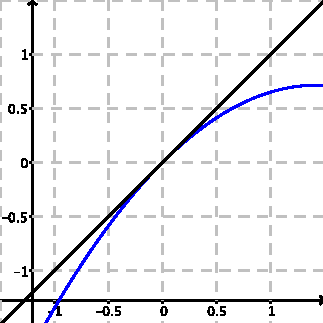
\includegraphics[scale=0.8]{figures/roots-fixedpt6} 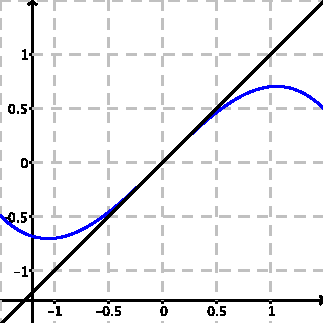
\includegraphics[scale=0.8]{figures/roots-fixedpt7}
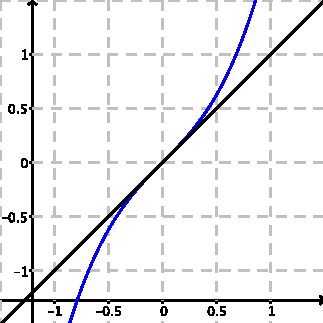
\includegraphics[scale=0.8]{figures/roots-fixedpt8}
\end{figure}
\par\end{center}

\noindent Pada salah satu fungsi ini, iterasi titik tetap konvergen
untuk semua nilai dalam suatu lingkungan titik tetap. Pada fungsi
lainnya, iterasi titik tetap meninggalkan suatu lingkungan titik tetap
untuk semua nilai awal di lingkungan tersebut kecuali titik tetap
itu sendiri. Pada fungsi ketiga, iterasi titik tetap konvergen ke
titik tetap untuk beberapa nilai awal dan meninggalkan suatu lingkungan
titik tetap untuk nilai awal lainnya (dan \textit{setiap} lingkungan
titik tetap akan memuat kedua jenis nilai awal). Dapatkah Anda menentukan
yang mana? Temukan jawabannya dengan membuat diagram jaring untuk
masing-masing. Jawaban \vpageref{subsec:Answers-fixedPointIteration}.

Bukti Teorema Kekonvergenan Titik Tetap dapat dengan mudah diperluas
untuk mencakup nilai awal dalam sembarang lingkungan titik tetap tempat
nilai mutlak turunan tetap kurang dari $1$. Ukuran dan kesimetrian
interval tidak penting. Sebagai contoh, $f(x)=\frac{1}{8}x^{3}-x^{2}+2x+1$
memiliki titik tetap di $\hat{x}=2$. Bukti Teorema Kekonvergenan
Titik Tetap menetapkan kekonvergenan menuju $2$ dalam interval simetris
di sekitar $2$ misalnya $[1.9,2.1]$. Namun, interval ini jauh dari
lingkungan terbesar nilai-nilai awal yang membuat iterasi titik tetap
konvergen ke $2$. Kita dapat mencari batas-batas interval terbesar
semacam itu dengan menyelesaikan persamaan $|f'(x)|=1$. Untuk itu:
\begin{eqnarray*}
\frac{3}{8}x^{2}-2x+2 & = & \pm1\\
3x^{2}-16x+16 & = & \pm8\\
3x^{2}-16x+24=0 & atau & 3x^{2}-16x+8=0\\
x=\frac{8\pm i2\sqrt{2}}{3} & atau & x=\frac{8\pm2\sqrt{10}}{3}\\
\frac{8-2\sqrt{10}}{3}\approx0.558 & dan & \frac{8+2\sqrt{10}}{3}\approx4.775,
\end{eqnarray*}
Jadi, kita patut mengharapkan iterasi titik tetap konvergen ke 2 pada
setiap interval tertutup yang termuat dalam
\[
\left(\frac{8-2\sqrt{10}}{3},\frac{8+2\sqrt{10}}{3}\right).
\]
 Sekarang, jika kita meminta komputer menjalankan iterasi titik tetap
untuk sejumlah besar nilai awal yang berjarak sama, misalnya 100 nilai,
pada interval $[-2,8]$ lalu mencatat hasilnya pada garis bilangan
dengan mewarnai suatu nilai awal hitam jika tidak konvergen ke 2 dan
hijau jika konvergen ke 2 (diagram semacam itu akan kita sebut diagram
kekonvergenan), kita memperoleh

\begin{center}
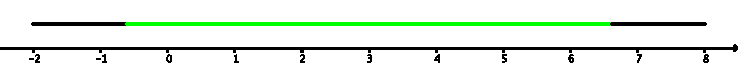
\includegraphics{figures/roots-fixedpt9},
\par\end{center}

\noindent yang menunjukkan bahwa iterasi titik tetap konvergen ke
2 untuk nilai awal pada interval kira-kira $[-0.5,6.5]$. Memang,
eksperimen tersebut menegaskan bahwa iterasi titik tetap konvergen
pada setiap interval tertutup yang termuat dalam $\left(\frac{8-2\sqrt{10}}{3},\frac{8+2\sqrt{10}}{3}\right)$
sebagaimana diprediksi. Namun, diagram itu menunjukkan kekonvergenan
pada himpunan yang bahkan lebih besar. Kita dapat menyimpulkan bahwa
Teorema Kekonvergenan Titik Tetap memberikan syarat yang cukup, tetapi
bukan syarat yang perlu, bagi kekonvergenan dalam suatu lingkungan
titik tetap. 

Grafik fungsi $f(x)$ yang ditumpangtindihkan dengan garis $y=x$
(Gambar \ref{fig:basinOfAttractionExplanation}) 
\begin{figure}
\caption{\label{fig:basinOfAttractionExplanation}$f(x)=\frac{1}{8}x^{3}-x^{2}+2x+1$
dan garis $y=x$}

\centering{}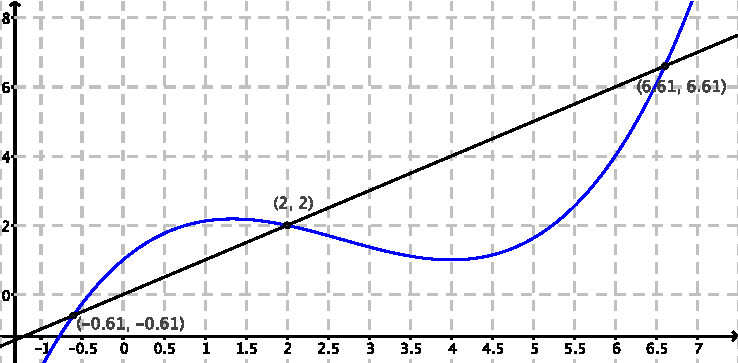
\includegraphics{figures/roots-fixedpt10}
\end{figure}
 memberi gambaran mengapa batas $\frac{8\pm2\sqrt{10}}{3}$ belum
menceritakan keseluruhan keadaan. Dengan membayangkan diagram jaring
untuk sembarang nilai awal di antara dua titik tetap selain 2, yakni
$-0.61$ dan $6.61$, Anda seharusnya dapat meyakinkan diri bahwa
iterasi titik tetap konvergen ke $2$ untuk sembarang nilai awal dalam
interval $(-0.61,6.61)$. Dapatkah Anda membuktikannya? Grafik seperti
dalam Gambar \ref{fig:fixed-pt-zoom}, \ref{fig:derivativeEqualsOne},
dan \ref{fig:basinOfAttractionExplanation} sangat diperlukan dan
harus selalu diperiksa ketika mencoba memahami iterasi titik tetap,
tetapi grafik tersebut tidak boleh dijadikan bukti. Untuk pembuktian,
kita perlu mengandalkan teorema seperti Teorema Kekonvergenan Titik
Tetap.

\noindent\begin{digression}{Sebuah kuadrat yang menarik} 

\noindent Mencoba mencari akar persamaan logistik 
\[
g(x)=(\alpha-1)x-\alpha x^{2}
\]
dengan menerapkan iterasi titik tetap pada fungsi yang bersesuaian
$f(x)=x+g(x)=\alpha x(1-x)$ merupakan latihan terkenal dalam sistem
dinamis, tetapi cara ini terkenal sering tidak berhasil! Selesaikan
penyelidikan berikut untuk melihat apa yang terjadi.
\begin{enumerate}
\item Tunjukkan bahwa $f(x)=\alpha x(1-x)$ seperti yang dinyatakan.
\item Untuk setiap nilai $\alpha=2.5$, $\alpha=3.2$, $\alpha=3.833$,
dan $\alpha=4$, lakukan langkah-langkah berikut.

\begin{enumerate}
\item Tentukan secara analitis titik tetap positif dari $f$ (akar $g$)
(dengan pensil, kertas, dan sedikit aljabar). 
\item Tetapkan $x_{0}=0.1$ dan gunakan program komputer untuk menghitung
$x_{975}$ sampai $x_{1000}$.
\item Amati 26 hasil iterasi pada bagian (b) dan jelaskan apa yang Anda
lihat.
\end{enumerate}
\item Hubungkan hasil yang Anda peroleh pada bagian 2 dengan diagram berikut.

\begin{center}
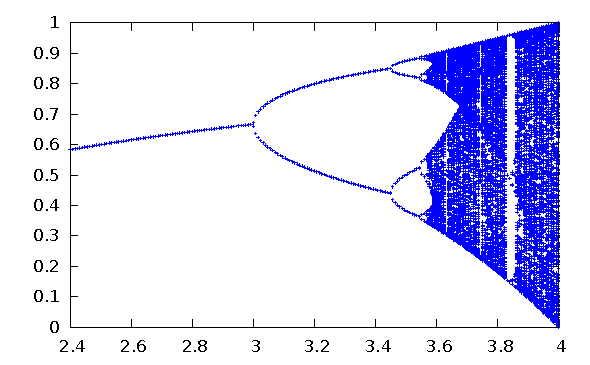
\includegraphics{figures/phaseDiagram}
\par\end{center}
\item Gunakan diagram tersebut untuk memperkirakan nilai $\alpha$ yang
menurut Anda akan membuat iterasi titik tetap menghasilkan $x_{975}$
sampai $x_{1000}$ yang berulang dalam siklus empat nilai berbeda.
Periksa perkiraan Anda.
\end{enumerate}
\noindent\end{digression}

\subsection{Pencarian Akar\label{subsec:RootFindingInvestigation}}

Jika berhasil, iterasi titik tetap menemukan solusi persamaan berbentuk
$f(x)=x$. Masalah pencarian akar menuntut solusi persamaan berbentuk
$g(x)=0$. Namun, persamaan $f(x)=x$ memiliki solusi yang persis
sama dengan persamaan $f(x)-x=0$, sehingga mencari titik tetap $f(x)$
ekuivalen dengan mencari akar $g(x)=f(x)-x$. Memang, contoh pencarian
titik tetap $f(x)=\frac{1}{8}x^{3}-x^{2}+2x+1$ dapat kita nyatakan
ulang sebagai masalah pencarian akar $g(x)=f(x)-x=\frac{1}{8}x^{3}-x^{2}+x+1$.
Akan tetapi, justru masalah sebaliknya jauh lebih umum. Kita dihadapkan
pada masalah mencari akar suatu fungsi dan perlu menyatakannya ulang
sebagai masalah titik tetap.

Misalkan kita ingin mencari akar $g(x)=-x^{3}+5x^{2}-4x-6$. Pertanyaan
untuk menyelesaikan $g(x)=0$ dapat kita nyatakan ulang sebagai masalah
mencari titik tetap dari banyak fungsi yang berbeda! Namun, untuk
menurunkan fungsi-fungsi itu, Anda harus mengabaikan beberapa nasihat
bijak guru aljabar Anda! Kuncinya adalah menggunakan aljabar untuk
menulis ulang persamaan $-x^{3}+5x^{2}-4x-6=0$ sebagai persamaan
berbentuk $x=f(x)$. Cara paling sederhana adalah menambahkan $x$
pada kedua ruas persamaan. Manipulasi ini dan beberapa manipulasi
lainnya ditunjukkan dalam daftar berikut.
\begin{itemize}
\item $-x^{3}+5x^{2}-4x-6=0\Rightarrow-x^{3}+5x^{2}-3x-6=x$
\item $-x^{3}+5x^{2}-4x-6=0\Rightarrow-x^{3}+5x^{2}-6=4x\Rightarrow\frac{-x^{3}+5x^{2}-6}{4}=x$
\item $-x^{3}+5x^{2}-4x-6=0\Rightarrow-x^{3}-4x-6=-5x^{2}\Rightarrow\frac{x^{3}+4x+6}{5}=x^{2}\Rightarrow\pm\sqrt{\frac{x^{3}+4x+6}{5}}=x$
\item $-x^{3}+5x^{2}-4x-6=0\Rightarrow5x^{2}-4x-6=x^{3}\Rightarrow\sqrt[3]{5x^{2}-4x-6}=x$
\end{itemize}
Dapatkah Anda melihat apa yang dilakukan pada masing-masing baris?
Dengan demikian, kita memiliki lima kandidat untuk iterasi titik tetap,
$f_{1}(x)=-x^{3}+5x^{2}-3x-6$, $f_{2}(x)=\frac{-x^{3}+5x^{2}-6}{4}$,
$f_{3}(x)=\sqrt{\frac{x^{3}+4x+6}{5}}$, $f_{4}(x)=-\sqrt{\frac{x^{3}+4x+6}{5}}$,
dan $f_{5}(x)=\sqrt[3]{5x^{2}-4x-6}$, yang semuanya berpotensi menghasilkan
akar $g(x)$. Ada fungsi keenam yang akan kita bahas jauh lebih rinci
nanti: $f_{6}(x)=\frac{2x^{3}\text{\textminus}5x^{2}\text{\textminus}6}{3x^{2}\text{\textminus}10x+4}$\footnote{Dengan menghitung $f_{6}(1-\sqrt{3})$, $f_{6}(1+\sqrt{3})$, dan
$f_{6}(3)$, Anda dapat memverifikasi bahwa $f_{6}$ juga memiliki
ketiga nilai ini sebagai titik tetap.}. 
\begin{figure}
\caption{\label{fig:SixConvergenceDiagrams}Diagram kekonvergenan bagi 6 fungsi
dengan titik tetap yang sama.}

\bigskip{}

\begin{centering}
$f_{1}$: 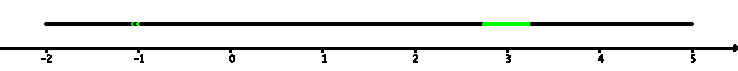
\includegraphics{figures/roots-fixedpt11}
\par\end{centering}
\begin{centering}
$f_{2}$: 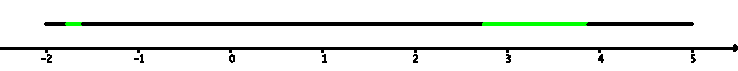
\includegraphics{figures/roots-fixedpt12}
\par\end{centering}
\begin{centering}
$f_{3}$: 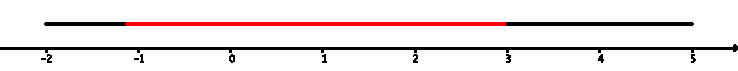
\includegraphics{figures/roots-fixedpt13}
\par\end{centering}
\begin{centering}
$f_{4}$: 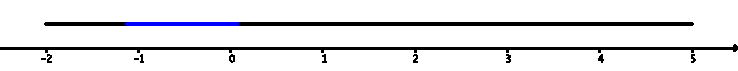
\includegraphics{figures/roots-fixedpt14}
\par\end{centering}
\begin{centering}
$f_{5}$: 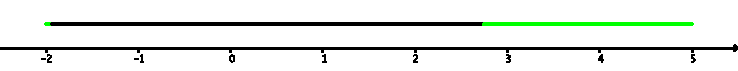
\includegraphics{figures/roots-fixedpt15}
\par\end{centering}
\begin{centering}
$f_{6}$: 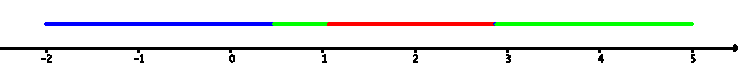
\includegraphics{figures/roots-fixedpt16}
\par\end{centering}
\centering{}hitam: tidak konvergen; hijau: konvergen ke $3$; merah:
konvergen ke $1+\sqrt{3}$; biru: konvergen ke $1-\sqrt{3}$
\end{figure}
 Akar-akar $g(x)$ adalah $1-\sqrt{3}\approx-0.73$, $1+\sqrt{3}\approx2.73$,
dan $3$, sehingga kita akan meninjau diagram kekonvergenan pada interval
$[-2,5]$. Iterasi titik tetap konvergen ke titik tetap yang berbeda
untuk fungsi yang berbeda meskipun keenam fungsi memiliki tepat tiga
titik tetap yang sama. Diagram kekonvergenan pada Gambar \ref{fig:SixConvergenceDiagrams}
diberi kode warna untuk menggambarkan kenyataan ini. Seperti sebelumnya,
warna hitam menunjukkan ketakkonvergenan. Warna hijau, merah, dan
biru masing-masing menunjukkan kekonvergenan ke $3$, $1+\sqrt{3}$,
dan $1-\sqrt{3}$, secara berurutan. Perhatikan bahwa hanya $f_{6}$
yang menghasilkan kekonvergenan, sejauh yang dapat kita ketahui, untuk
setiap nilai awal dalam $[-2,5]$, dan fungsi ini juga merupakan satu-satunya
fungsi yang membuat iterasi titik tetap konvergen ke titik tetap berbeda
untuk nilai awal berbeda. Cobalah memahami alasan perilaku kekonvergenan
setiap fungsi dengan mengamati grafik $f_{1},f_{2},\ldots,f_{6}$.
Berikan perhatian khusus pada grafik di sekitar $1+\sqrt{3}$ dan
$3$. Tampilan grafik dapat menyesatkan di daerah itu karena kedua
titik tetap sangat berdekatan. Coba juga temukan dua nilai awal dalam
$[-2,5]$ yang menyebabkan iterasi titik tetap dengan $f_{6}$ tidak
konvergen. Lalu, apa yang terjadi? Sebagai tantangan tambahan, cobalah
menemukan nilai ketiga dalam $[-2,5]$ yang menyebabkan iterasi titik
tetap dengan $f_{6}$ tidak konvergen. Petunjuk: Anda mungkin perlu
menggunakan sistem aljabar komputer untuk menemukan nilai semacam
itu secara eksak, atau menggunakan iterasi titik tetap untuk menghampirinya!
Jawaban \vpageref{subsec:Answers-fixedPointIteration}.

\subsection{Metode Iterasi Titik Tetap (kode semu)\index{metode iterasi titik tetap!kode semu}}

Meskipun kita telah banyak membahas cara menentukan apakah metode
iterasi titik tetap diperkirakan akan konvergen atau tidak, tak satu
pun informasi tersebut diperlukan secara langsung untuk mengodekan
metode itu. Setiap implementasi metode ini harus memungkinkan pengguna
mencoba iterasi titik tetap untuk sembarang fungsi dengan sembarang
nilai awal. Pengguna bertanggung jawab memahami bahwa ketika asumsi-asumsinya
tidak terpenuhi, hasilnya tidak dapat diprediksi. Ingat, ``sampah
masuk...sampah keluar.''

Metode iterasi titik tetap menimbulkan masalah yang tidak terdapat
pada metode bagi dua. Dalam metode bagi dua, terdapat rumus yang sederhana
dan praktis untuk batas atas galat. Untuk menyediakan hal serupa dalam
metode iterasi titik tetap, kita harus mengorbankan kesederhanaan,
kepraktisan, atau keduanya, sedangkan manfaatnya tidak sebanding dengan
pengorbanan tersebut. Sebagai gantinya, digunakan kriteria penghentian
yang lebih umum. Ketika dua nilai iterasi berturut-turut lebih dekat
satu sama lain daripada toleransi yang diberikan, metode berhenti.
Pada saat itu, selisih antara nilai iterasi, katakanlah $x_{k}$ dan
$x_{k+1}$, lebih kecil daripada toleransi. Untuk barisan yang dihasilkan
oleh iterasi titik tetap, $x_{k+1}=f(x_{k})$, sehingga $|x_{k+1}-x_{k}|=|f(x_{k})-x_{k}|$.
Ketika $|x_{k+1}-x_{k}|$ kecil, $|f(x_{k})-x_{k}|$ juga kecil, sehingga
$f(x_{k})\approx x_{k}$. $x_{k}$ ``hampir'' merupakan titik tetap.

\begin{pseudocode} 
\begin{description}
\item [{Asumsi:}] $f$ terdiferensialkan. $f$ mempunyai titik tetap $\hat{x}$.
$x_{0}$ berada dalam lingkungan $(\hat{x}-\delta,\hat{x}+\delta)$
tempat nilai mutlak $f'$ kurang dari satu.
\item [{Masukan:}] Nilai awal $x_{0}$; fungsi $f$; akurasi yang diinginkan
$tol$; jumlah maksimum iterasi $N$.
\item [{Langkah~1:}] Untuk $j=1\ldots N$ lakukan Langkah 2-4:

\begin{description}
\item [{Langkah~2:}] Tetapkan $x=f(x_{0})$;
\item [{Langkah~3:}] Jika $|x-x_{0}|\leq tol$ maka kembalikan $x$;
\item [{Langkah~4:}] Tetapkan $x_{0}=x$;
\end{description}
\item [{Langkah~5:}] Cetak ``Metode gagal. Jumlah maksimum iterasi terlampaui.''
\item [{Keluaran:}] Hampiran $x$ yang mendekati titik tetap eksak, atau
pesan kegagalan.
\end{description}
\end{pseudocode}  

\subsection{Konsep Utama}
\begin{description}
\item [{Titik~tetap:}] $x_{0}$ adalah titik tetap fungsi $f(x)$ jika
$f(x_{0})=x_{0}$.
\item [{Iterasi~titik~tetap:}] \index{metode iterasi titik tetap} Menghitung
barisan $x_{0},x_{1}=f(x_{0}),x_{2}=f(x_{1}),x_{3}=f(x_{2}),\ldots$
berdasarkan fungsi $f$ dan nilai awal $x_{0}$.
\item [{Titik~tetap~atraktif:}] Suatu titik tetap disebut \index{titik tetap!atraktif}
atraktif (atau penarik) jika terdapat lingkungan titik tetap tersebut
yang membuat iterasi titik tetap konvergen untuk semua nilai awal
di dalam lingkungan itu.
\item [{Titik~tetap~repulsif:}] Suatu titik tetap disebut \index{titik tetap!repulsif}
repulsif (atau penolak) jika iterasi titik tetap meninggalkan suatu
lingkungan titik tetap tersebut untuk sembarang nilai awal di dalam
lingkungan itu selain titik tetap itu sendiri.
\item [{Teorema~Nilai~Rata-Rata:}] \index{Teorema!Nilai Rata-Rata}Jika
$f$ kontinu pada $[a,b]$ dan dapat didiferensialkan pada $(a,b)$,
maka terdapat $c\in(a,b)$ sedemikian sehingga $f'(c)=\frac{f(b)-f(a)}{b-a}$.
\item [{Teorema~Kekonvergenan~Titik~Tetap:}] \index{Teorema!Kekonvergenan Titik Tetap}
Diberikan suatu fungsi $f(x)$ dengan turunan pertama yang kontinu
dan titik tetap $\hat{x}$, jika $|f'(\hat{x})|<1$ maka terdapat
suatu lingkungan $\hat{x}$ tempat iterasi titik tetap konvergen ke
titik tetap tersebut untuk setiap nilai awal dalam lingkungan itu.
\end{description}
\startexercises

\subsection{Latihan}
\begin{enumerate}
\item \label{enu:fixedPtIterationCode}Tulislah fungsi Octave yang mengimplementasikan
metode iterasi titik tetap. Simpan fungsi tersebut sebagai berkas
\texttt{.m} untuk digunakan di kemudian hari.
\item \label{enu:mvtExamples}(i) Tentukan apakah fungsi pada interval tersebut
memenuhi hipotesis Teorema Nilai Rata-Rata. (ii) Jika hipotesis terpenuhi,
carilah nilai $c$ yang keberadaannya dijamin oleh teorema tersebut.

\begin{enumerate}
\item $f(x)=3-x-\sin x$; $[2,3]$
\item $g(x)=3x^{4}-2x^{3}-3x+2$; $[0,1]$
\item \label{exc:fixedpt}$g(x)=3x^{4}-2x^{3}-3x+2$; $[0,0.9]$ \hasasolution 
\item \label{exc:fixedpt-16}$h(x)=10-\cosh(x)$; $[-3,-2]$ \hasananswer 
\item $f(t)=\sqrt{4+5\sin t}-2.5$; $[-6,-5]$
\item \label{exc:fixedpt-1}$g(t)=\frac{3t^{2}\tan t}{1-t^{2}}$; $[20,23]$ \hasasolution 
\item \label{exc:fixedpt-2}$h(t)=\ln(3\sin t)-\frac{3t}{5}$; $[2,4]$ \hasananswer 
\item \label{exc:fixedpt-3}$f(r)=e^{\sin r}-r$; $[-20,20]$ \hasananswer 
\item $g(r)=\sin(e^{r})+r$; $[-3,3]$
\item $h(r)=2^{\sin r}-3^{\cos r}$; $[1,3]$
\end{enumerate}
\item Carilah semua titik tetap fungsi tersebut secara eksak. Gunakan aljabar.

\begin{enumerate}
\item $f(x)=\sqrt[3]{2x^{3}-x^{2}-x}$
\item $f(x)=\frac{\ln(2e^{x})}{2}$
\item \label{exc:fixedpt-4}$f(x)=\log(x^{2}-3x)-1+x$ \hasananswer 
\item \label{exc:fixedpt-5}$g(x)=3x^{2}+5x+1$ \hasananswer 
\item $g(t)=t+\frac{5000}{1+2e^{-3t}}-2500$
\item $g(x)=e^{\ln(x+1)-3}$
\item $h(x)=\sqrt{4x^{2}+4x+1}$
\item \label{exc:fixedpt-6}$h(x)=x-10+3^{x}+25\cdot3^{-x}$ \hasasolution 
\item $h(x)=x+6-3\log_{5}(2x)$
\end{enumerate}
\item Carilah setidaknya dua fungsi kandidat, $f_{1}(x)$ dan $f_{2}(x)$,
untuk mencari akar $g(x)$ melalui iterasi titik tetap. Dengan kata
lain, ubah masalah mencari akar $g$ menjadi masalah mencari titik
tetap $f_{1}$ atau $f_{2}$.

\begin{enumerate}
\item $g(x)=7x^{2}+5x-9$
\item $g(x)=x+\cos x$
\item \label{exc:fixedpt-7}$g(x)=6x^{5}+12x^{2}-8$ \hasananswer 
\item \label{exc:fixedpt-8}$g(x)=x^{2}-e^{3x+4}$ \hasasolution 
\item $g(x)=7x-3\cos(\pi x-2)+\ln|2x^{2}+4x-8|$
\item \label{exc:fixedpt-9}$g(x)=3^{x^{2}-5x+1}-2^{-x^{2}-5x-1}$ \hasananswer 
\end{enumerate}
\item \label{enu:fixedPtIterationExamples}Hitung 5 iterasi pertama metode
iterasi titik tetap dengan menggunakan fungsi dan nilai awal yang
diberikan. Berdasarkan kelima iterasi ini, apakah Anda memperkirakan
metode tersebut akan konvergen?

\begin{enumerate}
\item $f(x)=3-\sin x$; $x_{0}=2$
\item \label{exc:fixedpt-10}$g(x)=10+x-\cosh(x)$; $x_{0}=-3$ \hasasolution 
\item \label{exc:fixedpt-11}$h(t)=\ln(3\sin t)+\frac{2t}{5}$; $t_{0}=1$ \hasananswer 
\item $w(r)=2^{\sin r}-3^{\cos r}+r$; $r_{0}=1$
\end{enumerate}
\item \label{enu:usingOctave}Gunakan fungsi Octave Anda dari soal \ref{enu:fixedPtIterationCode}
untuk setiap pasangan fungsi dan nilai awal pada soal \ref{enu:fixedPtIterationExamples}.
Atur toleransi menjadi $10^{-10}$ dan jumlah maksimum iterasi menjadi
100. Untuk setiap pasangan, apakah metode tersebut konvergen dalam
paling banyak 100 iterasi? Jika ya, ke nilai berapa? Laporkan setidaknya
10 angka signifikan. \haspartwithsolution  \haspartwithanswer 
\item \label{enu:usingWeb}Buatlah diagram jaring untuk setiap pasangan
fungsi/nilai awal pada soal \ref{enu:fixedPtIterationExamples}. \haspartwithsolution  \haspartwithanswer 
\item Bandingkan hasil dari soal \ref{enu:usingOctave} dengan hasil dari
soal \ref{enu:usingWeb}. Apakah keduanya konsisten?
\item Gunakan Proposisi \ref{prop:uniquenessOfFixedPoint} untuk menunjukkan
bahwa $g(x)=2x(1-x)$ mempunyai tepat satu titik tetap pada $[0.3,0.7]$.
\item \label{exc:fixedpt-12}Misalkan $f(x)=\frac{3x^{2}\text{\textminus}1}{6x+4}$. \hasasolution 

\begin{enumerate}
\item Tunjukkan bahwa $f$ mempunyai tepat satu titik tetap pada $[-4,-0.9]$.
\item Gunakan iterasi titik tetap untuk mencari hampiran titik tetap dengan
galat tidak lebih dari $10^{-2}$.
\end{enumerate}
\item \label{enu:ShowPart2}Misalkan $g(x)=\pi+0.5\sin(x/2)$.

\begin{enumerate}
\item Tunjukkan bahwa $g$ mempunyai tepat satu titik tetap pada $[0,2\pi]$. 
\item Gunakan iterasi titik tetap untuk mencari hampiran titik tetap dengan
galat tidak lebih dari $10^{-2}$.
\end{enumerate}
\item \label{exc:fixedpt-13}Tunjukkan bahwa metode iterasi titik tetap
yang diterapkan pada $f(x)=\sqrt[3]{8-4x}$ akan konvergen ke suatu
akar $g(x)=x^{3}+4x-8$ untuk setiap nilai awal $x_{0}\in[1.2,1.5]$. \hasasolution 
\item Tunjukkan bahwa iterasi titik tetap dijamin konvergen ke titik tetap
dari
\[
f(x)=(\sqrt{2})^{x}
\]
untuk setiap $x_{0}\in[1,3]$. PETUNJUK: $f'(x)=\frac{1}{2}\ln(2)\cdot(\sqrt{2})^{x}$.
\item Misalkan $g(x)=x^{2}-3x-2$. 

\begin{enumerate}
\item Carilah fungsi $f$ yang membuat iterasi titik tetap konvergen ke
suatu akar $g$. 
\item Gunakan fungsi tersebut untuk mencari akar $g$ dengan galat tidak
lebih dari $10^{-3}$ dari nilai eksaknya.
\item Nyatakan nilai awal yang Anda gunakan dan banyaknya iterasi yang diperlukan
untuk memperoleh hampiran tersebut.
\end{enumerate}
\item Gunakan iterasi titik tetap dengan $p_{0}=-1$ untuk menghampiri akar
$g(x)=x^{3}-3x+3$ hingga ketelitian $10^{-4}$.
\item Gunakan suatu metode iterasi titik tetap untuk mencari hampiran $\sqrt{3}$
dengan galat tidak lebih dari $10^{-4}$. Fungsi Anda hanya boleh
menggunakan konstanta bilangan bulat. Fungsi dan nilai awal apa yang
Anda gunakan?
\item Fungsi $g(x)=x^{4}+2x^{2}-x-3$ mempunyai dua akar. Salah satunya
berada dalam $[-1,0]$ dan yang lainnya berada dalam $[1,2]$.

\begin{enumerate}
\item Sebagai persiapan untuk mencari akar $g(x)$ dengan iterasi titik
tetap, salah satu cara memanipulasi persamaan $x^{4}+2x^{2}-x-3=0$
adalah dengan menambahkan $x$ pada kedua ruas. Hasilnya
\[
x=x^{4}+2x^{2}-3
\]
Buatlah grafik yang sesuai untuk menentukan apakah iterasi fungsi
$f(x)=x^{4}+2x^{2}-3$ akan menemukan akar dalam $[-1,0]$. Bagaimana
dengan akar dalam $[1,2]$? Jelaskan bagaimana Anda memperoleh kesimpulan
tersebut.
\item \label{root1}Manipulasilah persamaan $x^{4}+2x^{2}-x-3=0$ sedemikian
rupa sehingga iterasi titik tetap berhasil menemukan akar dalam $[-1,0]$.
Gambarlah grafik yang menunjukkan bahwa metode Anda akan berhasil.
\item \label{root2}Apakah manipulasi yang sama memungkinkan Anda menemukan
akar dalam $[1,2]$? Jika tidak, carilah manipulasi lain yang dapat
melakukannya. Sekali lagi, tampilkan grafik yang menunjukkan bahwa
metode Anda akan berhasil.
\item Gunakan metode Anda dari bagian \ref{root1} dan \ref{root2} untuk
mencari kedua akar hingga 3 tempat desimal.
\end{enumerate}
\item \label{exc:fixedpt-14}Iterasi titik tetap pada $f(x)=\sqrt[3]{2x^{3}-x^{2}-x}$
tidak akan konvergen ke suatu titik tetap. Akan tetapi, iterasi titik
tetap pada fungsi $g(x)=\sqrt[3]{x^{2}+x}$ akan konvergen kira-kira
ke $1.618033988749895$ untuk setiap $x_{0}$ dalam $[0.5,3.5]$. \hasananswer 

\begin{enumerate}
\item Berapa banyak iterasi yang diperlukan untuk mencapai akurasi $10^{-4}$
dengan menggunakan $g(x)$ dengan $x_{0}=2.5$?
\item Jelaskan mengapa $f(x)$ dan $g(x)$ mempunyai titik-titik tetap yang
sama.
\end{enumerate}
\item Carilah satu nol (nol mana pun) dari $g(x)=x^{2}+10\cos x$ dengan
galat tidak lebih dari $10^{-4}$ menggunakan iterasi titik tetap.
Nyatakan:

\begin{enumerate}
\item fungsi $f$ yang Anda gunakan dalam iterasi titik tetap
\item nilai awal, $x_{0}$, yang Anda gunakan
\item jumlah iterasi yang diperlukan
\end{enumerate}
\item \label{enu:fixedExp}Misalkan $c$ adalah bilangan real tak nol. Tunjukkan
bahwa setiap titik tetap tak nol dari $f(x)=xe^{c\cdot g(x)}$ merupakan
akar dari $g$.
\item Hampiri $\sqrt{3}$ dengan metode yang disarankan oleh soal \ref{enu:fixedExp}.
\item \label{enu:findC}Misalkan $g(\hat{x})=0$, $g$ memiliki turunan
pertama yang kontinu, dan $g'(\hat{x})\neq0$. Tunjukkan bahwa terdapat
suatu nilai $c$ sehingga iterasi titik tetap pada $f(x)=x+cg(x)$
konvergen ke $\hat{x}$ dalam suatu lingkungan $\hat{x}$.
\item \label{exc:fixedpt-15}Tentukan nilai $c$ yang menjamin bahwa iterasi
titik tetap untuk fungsi $f(x)=x+c(x-5\cos x)$ konvergen dari sembarang
nilai awal $x_{0}\in[0,\pi/2]$. Jelaskan. \hasananswer 
\item Misalkan $g(x)=$$\frac{1}{2}^{x}+\frac{1}{5}^{x}-10^{-5}$. 

\begin{enumerate}
\item Tunjukkan bahwa jika $g(x)$ memiliki nol di $p$, maka fungsi $f(x)=x+cg(x)$
memiliki titik tetap di $p$.
\item \label{findc}Tentukan nilai $c$ sehingga iterasi titik tetap pada
$f(x)$ konvergen untuk setiap nilai awal, $p_{0}$, dalam interval
$[16,17]$. Buat sketsa grafik yang menunjukkan bahwa pilihan $c$
Anda tepat.
\item Gunakan fungsi dari bagian \ref{findc} dengan nilai $c$ yang telah
Anda tentukan untuk mencari akar $g(x)$ yang akurat hingga $10^{-4}$.
Nyatakan nilai yang Anda gunakan untuk $p_{0}$. Tunjukkan tiga iterasi
terakhir. Berapa iterasi yang diperlukan?
\end{enumerate}
\item Buktikan bahwa untuk $f(x)=\cos x$, iterasi titik tetap konvergen
untuk setiap nilai awal.
\item \label{enu:convergenceStrengthened}Teorema Kekonvergenan Titik Tetap
dapat diperkuat. Syarat bahwa turunan pertama harus kontinu dapat
diganti. Ubah bukti dalam teks untuk menunjukkan pernyataan berikut.

\textit{Diberikan suatu fungsi $f(x)$ yang dapat didiferensialkan
dengan titik tetap $\hat{x}$, jika $|f'(x)|\leq M<1$ untuk setiap
$x$ dalam suatu lingkungan $\hat{x}$, maka iterasi titik tetap konvergen
ke titik tetap tersebut untuk setiap nilai awal dalam lingkungan itu.}
\item Buat tiga grafik yang serupa dengan grafik pada Gambar \ref{fig:derivativeEqualsOne}
untuk menganalisis keadaan ketika turunan di titik tetap sama dengan
$-1$. Apakah keadaan itu berbeda dari keadaan ketika turunan di titik
tetap sama dengan $1$?
\end{enumerate}
\noindent\finishexercises

\subsection*{Jawaban\label{subsec:Answers-fixedPointIteration}}
\begin{description}
\item [{Gambar~\ref{fig:derivativeEqualsOne}:}] Dari kiri ke kanan: setiap
lingkungan titik tetap memuat kedua jenis nilai awal; iterasi titik
tetap konvergen untuk semua nilai dalam suatu lingkungan titik tetap;
iterasi titik tetap meninggalkan suatu lingkungan titik tetap untuk
semua nilai awal dalam lingkungan itu kecuali titik tetap itu sendiri.
\item [{Gambar~\ref{fig:SixConvergenceDiagrams}:}] Ketika penyebutnya
nol, $f_{6}(x)$ tidak terdefinisi (terdapat asimtot vertikal pada
grafik), sehingga kita menyelesaikan $3x^{2}\text{\textminus}10x+4=0$
untuk memperoleh dua nilai awal yang menyebabkan iterasi titik tetap
gagal (karena iterasi pertama tidak terdefinisi). Nilai-nilai itu
adalah $x=\frac{5\pm\sqrt{13}}{3}\approx.4648\mbox{ dan }2.868$.
Untuk mencari titik ketiga yang menyebabkan iterasi titik tetap gagal,
kita menyelesaikan persamaan $f_{6}(x)=\frac{5+\sqrt{13}}{5}$ (kita
juga dapat menyelesaikan $f_{6}(x)=\frac{5-\sqrt{13}}{5}$ sebagai
gantinya). Maka iterasi kedua tidak terdefinisi karena iterasi pertama
menghasilkan $\frac{5+\sqrt{13}}{5}$. Satu-satunya solusi real kira-kira
$1.055909763230534$, yang dapat ditemukan melalui iterasi titik tetap
pada $\sqrt[3]{\frac{\sqrt{13}x^{2}+10x^{2}\text{\textminus}\frac{10\sqrt{13}x}{3}\text{\textminus}\frac{50x}{3}+\frac{4\sqrt{13}}{3}+\frac{38}{3}}{2}}$.
Buktikan. Namun, perhatikan bahwa pernyataan bahwa iterasi titik tetap
akan gagal didasarkan pada asumsi aritmetika \textit{eksak}. Fakta
bahwa setiap implementasi wajar metode iterasi titik tetap akan melibatkan
aritmetika titik mengambang dapat menimbulkan galat yang cukup besar
sehingga metode tersebut konvergen bahkan untuk nilai-nilai awal ini.
\end{description}

